%%%%%%%%%%%%%%%%%%%%%%%%%%%%%%%%%%%%%%%%%
% Simple Sectioned Essay Template
% LaTeX Template
%
% This template has been downloaded from:
% http://www.latextemplates.com
%
% Note:
% The \lipsum[#] commands throughout this template generate dummy text
% to fill the template out. These commands should all be removed when 
% writing essay content.
%
%%%%%%%%%%%%%%%%%%%%%%%%%%%%%%%%%%%%%%%%%

%----------------------------------------------------------------------------------------
%	PACKAGES AND OTHER DOCUMENT CONFIGURATIONS
%----------------------------------------------------------------------------------------

\documentclass[12pt]{article} % Default font size is 12pt, it can be changed here

\usepackage{geometry} % Required to change the page size to A4
\geometry{a4paper} % Set the page size to be A4 as opposed to the default US Letter

\usepackage{graphicx} % Required for including pictures

\usepackage{float} % Allows putting an [H] in \begin{figure} to specify the exact location of the figure
\usepackage{wrapfig} % Allows in-line images such as the example fish picture

\usepackage{lipsum} % Used for inserting dummy 'Lorem ipsum' text into the template

\usepackage{url}

\linespread{1.2} % Line spacing

%\setlength\parindent{0pt} % Uncomment to remove all indentation from paragraphs

\graphicspath{{./figures/}} % Specifies the directory where pictures are stored

\begin{document}

%----------------------------------------------------------------------------------------
%	TITLE PAGE
%----------------------------------------------------------------------------------------

\begin{titlepage}

\newcommand{\HRule}{\rule{\linewidth}{0.5mm}} % Defines a new command for the horizontal lines, change thickness here

\center % Center everything on the page

\HRule \\[0.4cm]
{ \huge \bfseries Database Query Acceleration with Reconfigurable Computing Fabrics}\\[0.4cm] % Title of your document
\HRule \\[1.5cm]

\begin{minipage}{0.4\textwidth}
    \centering {Cheng Liu} \\ 
    \vspace{2em}
    \centering {\large \today}
\end{minipage}

\end{titlepage}

%----------------------------------------------------------------------------------------
%	TABLE OF CONTENTS
%----------------------------------------------------------------------------------------

%\tableofcontents % Include a table of contents

%\newpage % Begins the essay on a new page instead of on the same page as the table of contents 

%----------------------------------------------------------------------------------------
%	INTRODUCTION
%----------------------------------------------------------------------------------------
\section{Motivation} % Major section
FPGAs have been used as accelerators for high performance relation database applications. Compared
to other parallel computing architectures such as multi-core processors and GPUs, FPGAs usually
outperform on energy efficiency and can also achieve comparable performance in many cases. The
use of FPGAs for database acceleration now has attracted increasing attentions of database researchers
from both academia and industry. 

Most of the previous work focused on building specific circuits for the typical
compute-intensive operations involved in database query applications using either hardware description languages
(HDLs) or high level synthesis (HLS) languages while leaving the hardware unchanged through the
application lifetime. This explores the use of FPGAs for specific hardware accelerator design
and will be good enough when the application doesn't change with time. However, there are many cases
that the required FPGA accelerators may change with time. 

For instances, the load of database query may change with time \cite{guotowards}
\cite{soundararajan2009dynamic} and different types of
operations are needed accordingly. On top of the system fluctuation, the same operation such as sort
operating on different attributes of the database which can be float, string, char or integer utilizes
diverse FPGA resources. Unlike general computing architectures (i.e. CPU and GPUs) which typically use the
same computing cores to handle all the different operations, FPGAs needs specific hardware for each
types of operations. Therefore, some of the operations implemented may only be used for a short period
of time while they may consume considerable hardware resources. In addition, some of the
combination of the operations may be more efficient than the separate implementations
\cite{sadoghi2012multi} \cite{chenaccelerating} and the combined
implementations will be better when they are frequently used in the applications. But separate
implementations will be preferred when the operations are not used at the same time. The mismatch
between the database query and the underlying FPGA accelerators may result in severe performance and power
efficiency degradation. 

FPGAs which allow multiple granularities of reconfiguration using runtime mode selection, partial reconfiguration
techniques or multiple FPGA contexts can be adapted to bridge the gap and provide hardware accelerators as needed or just enough for the sake of performance and power efficiency of database query applications.

\section{Main Idea}
The basic database query processing system as shown in Fig. 1 follows the architecture that is used
in omniDB \cite{zhang2013omnidb} while the data-parallel
primitives will be implemented on FPGA. From the perspective of omniDB, the FPGA is abstracted as a
library providing all kinds of efficient data parallel primitives. Each primitive may have multiple
instances implemented on the FPGA. All the primitives implemented on FPGAs are managed by a
primitive resource manager. The manager will allocate a sequence of primitives to the high level data query
operators. When there are abundant hardware primitives, the manager will allocate hardware operators
as needed which essentially make best use of spacial resources providing the best performance. When
there are only limited hardware primitives, the manager will provide just enough primitives to high
level operators which try to temporally reuse the hardware resources.   

\begin{figure}[H]
\centering
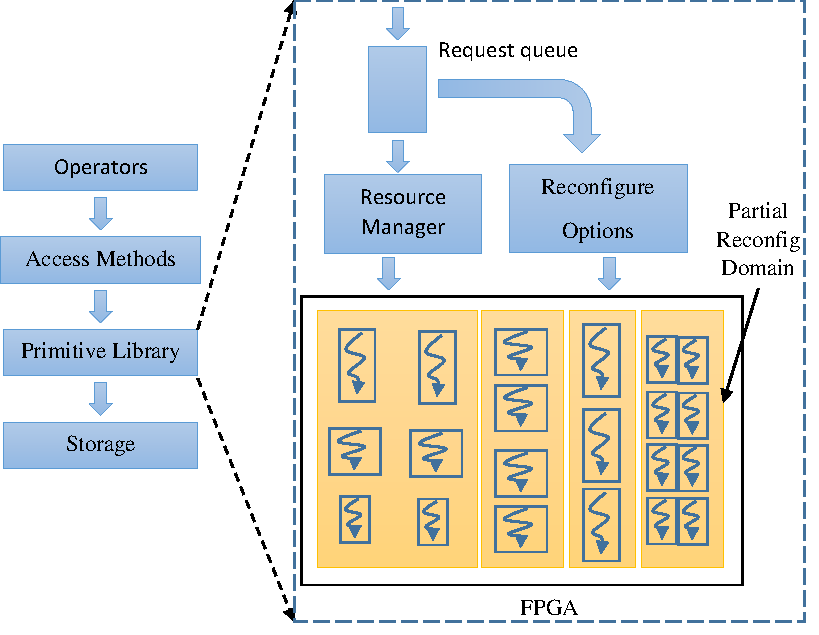
\includegraphics[width=10cm]{db-accelerator}
\caption{Database Processing Architecture Using FPGA Accelerators}
\label{fig:db-accelerator}
\end{figure}


To make best use of the hardware accelerators, a request queue will be maintained in the manager.
With the status of the queue, the underlying hardware primitives that will be needed can be analyzed
at runtime. Given this runtime information, the FPGAs can be reconfigured to match the requirements
at runtime using partial reconfigurations or some other dynamic reconfiguration techniques.
With some other high-level data query information, it is possible to reduce the frequency of the
runtime reconfiguration and thus are beneficial to the overall system. 

\subsection{How long does it take to reconfigure FPGA?}
There are typically three methods for FPGA reconfiguration as listed in Table 1 \cite{papadimitriou2011performance}. FPGA design with mode selection can
change its functionality by simply modifying some selection configuration bits. This mode achieves
the fastest configuration but it usually requires the design to include all the functionality. Thus
it typically results in large resource consumption. Multi-context bitstream method is relatively slow and
needs larger on-chip storage to keep the bitstream. In addition, it may need to reset the whole FPGA
board. Partial reconfiguration provides a nice trade-off between configuration time and on-chip
storage requirement. 
\begin{table}[!hbp]
    \centering
    \small
\begin{tabular}{c|c|c|c}
\hline
Reconfigure Method & mode selection & partial reconfiguration & multi-context bitstream \\
\hline
Reconfiguration Time & 1-10us & 1-100ms & 0.5-10s \\
\hline
Reconfiguration Size & 1-100B & 0.1-1000KB & 0.1-10MB \\
\hline
\end{tabular}
\caption{Reconfiguration Time}
\end{table} 


\subsection{Data query variation}
The authors in the papers \cite{guotowards}
\cite{soundararajan2009dynamic} motivated the dynamic resource management or allocation for database query
system. The analysis timescale is from seconds to minutes. I didn't see any report on
fine-grained analysis. Maybe I chose the inappropriate key words and more investigation will be
needed. If the database query varies in seconds, current FPGA reconfiguration capability should be
enough for runtime optimization.  


\section{Summary} 
Taking advantage of the FPGA's reconfigurability, the FPGA accelerators can be dynamically
reshaped to provide more hotspot acceleration fabrics based on the runtime requirements of data
query, which are beneficial to both the system's performance and power efficiency.

%----------------------------------------------------------------------------------------
%	BIBLIOGRAPHY
%----------------------------------------------------------------------------------------
\bibliographystyle{plain}
\bibliography{refs}
%----------------------------------------------------------------------------------------

\end{document}
